\documentclass[]{article}
\usepackage{lmodern}
\usepackage{amssymb,amsmath}
\usepackage{ifxetex,ifluatex}
\usepackage{fixltx2e} % provides \textsubscript
\ifnum 0\ifxetex 1\fi\ifluatex 1\fi=0 % if pdftex
  \usepackage[T1]{fontenc}
  \usepackage[utf8]{inputenc}
  \usepackage{eurosym}
\else % if luatex or xelatex
  \ifxetex
    \usepackage{mathspec}
  \else
    \usepackage{fontspec}
  \fi
  \defaultfontfeatures{Ligatures=TeX,Scale=MatchLowercase}
  \newcommand{\euro}{€}
\fi
% use upquote if available, for straight quotes in verbatim environments
\IfFileExists{upquote.sty}{\usepackage{upquote}}{}
% use microtype if available
\IfFileExists{microtype.sty}{%
\usepackage{microtype}
\UseMicrotypeSet[protrusion]{basicmath} % disable protrusion for tt fonts
}{}
\usepackage[margin=1in]{geometry}
\usepackage{hyperref}
\hypersetup{unicode=true,
            pdftitle={Inference 2 - Hypothesis Tests},
            pdfborder={0 0 0},
            breaklinks=true}
\urlstyle{same}  % don't use monospace font for urls
\usepackage{color}
\usepackage{fancyvrb}
\newcommand{\VerbBar}{|}
\newcommand{\VERB}{\Verb[commandchars=\\\{\}]}
\DefineVerbatimEnvironment{Highlighting}{Verbatim}{commandchars=\\\{\}}
% Add ',fontsize=\small' for more characters per line
\usepackage{framed}
\definecolor{shadecolor}{RGB}{248,248,248}
\newenvironment{Shaded}{\begin{snugshade}}{\end{snugshade}}
\newcommand{\KeywordTok}[1]{\textcolor[rgb]{0.13,0.29,0.53}{\textbf{#1}}}
\newcommand{\DataTypeTok}[1]{\textcolor[rgb]{0.13,0.29,0.53}{#1}}
\newcommand{\DecValTok}[1]{\textcolor[rgb]{0.00,0.00,0.81}{#1}}
\newcommand{\BaseNTok}[1]{\textcolor[rgb]{0.00,0.00,0.81}{#1}}
\newcommand{\FloatTok}[1]{\textcolor[rgb]{0.00,0.00,0.81}{#1}}
\newcommand{\ConstantTok}[1]{\textcolor[rgb]{0.00,0.00,0.00}{#1}}
\newcommand{\CharTok}[1]{\textcolor[rgb]{0.31,0.60,0.02}{#1}}
\newcommand{\SpecialCharTok}[1]{\textcolor[rgb]{0.00,0.00,0.00}{#1}}
\newcommand{\StringTok}[1]{\textcolor[rgb]{0.31,0.60,0.02}{#1}}
\newcommand{\VerbatimStringTok}[1]{\textcolor[rgb]{0.31,0.60,0.02}{#1}}
\newcommand{\SpecialStringTok}[1]{\textcolor[rgb]{0.31,0.60,0.02}{#1}}
\newcommand{\ImportTok}[1]{#1}
\newcommand{\CommentTok}[1]{\textcolor[rgb]{0.56,0.35,0.01}{\textit{#1}}}
\newcommand{\DocumentationTok}[1]{\textcolor[rgb]{0.56,0.35,0.01}{\textbf{\textit{#1}}}}
\newcommand{\AnnotationTok}[1]{\textcolor[rgb]{0.56,0.35,0.01}{\textbf{\textit{#1}}}}
\newcommand{\CommentVarTok}[1]{\textcolor[rgb]{0.56,0.35,0.01}{\textbf{\textit{#1}}}}
\newcommand{\OtherTok}[1]{\textcolor[rgb]{0.56,0.35,0.01}{#1}}
\newcommand{\FunctionTok}[1]{\textcolor[rgb]{0.00,0.00,0.00}{#1}}
\newcommand{\VariableTok}[1]{\textcolor[rgb]{0.00,0.00,0.00}{#1}}
\newcommand{\ControlFlowTok}[1]{\textcolor[rgb]{0.13,0.29,0.53}{\textbf{#1}}}
\newcommand{\OperatorTok}[1]{\textcolor[rgb]{0.81,0.36,0.00}{\textbf{#1}}}
\newcommand{\BuiltInTok}[1]{#1}
\newcommand{\ExtensionTok}[1]{#1}
\newcommand{\PreprocessorTok}[1]{\textcolor[rgb]{0.56,0.35,0.01}{\textit{#1}}}
\newcommand{\AttributeTok}[1]{\textcolor[rgb]{0.77,0.63,0.00}{#1}}
\newcommand{\RegionMarkerTok}[1]{#1}
\newcommand{\InformationTok}[1]{\textcolor[rgb]{0.56,0.35,0.01}{\textbf{\textit{#1}}}}
\newcommand{\WarningTok}[1]{\textcolor[rgb]{0.56,0.35,0.01}{\textbf{\textit{#1}}}}
\newcommand{\AlertTok}[1]{\textcolor[rgb]{0.94,0.16,0.16}{#1}}
\newcommand{\ErrorTok}[1]{\textcolor[rgb]{0.64,0.00,0.00}{\textbf{#1}}}
\newcommand{\NormalTok}[1]{#1}
\usepackage{graphicx,grffile}
\makeatletter
\def\maxwidth{\ifdim\Gin@nat@width>\linewidth\linewidth\else\Gin@nat@width\fi}
\def\maxheight{\ifdim\Gin@nat@height>\textheight\textheight\else\Gin@nat@height\fi}
\makeatother
% Scale images if necessary, so that they will not overflow the page
% margins by default, and it is still possible to overwrite the defaults
% using explicit options in \includegraphics[width, height, ...]{}
\setkeys{Gin}{width=\maxwidth,height=\maxheight,keepaspectratio}
\IfFileExists{parskip.sty}{%
\usepackage{parskip}
}{% else
\setlength{\parindent}{0pt}
\setlength{\parskip}{6pt plus 2pt minus 1pt}
}
\setlength{\emergencystretch}{3em}  % prevent overfull lines
\providecommand{\tightlist}{%
  \setlength{\itemsep}{0pt}\setlength{\parskip}{0pt}}
\setcounter{secnumdepth}{0}
% Redefines (sub)paragraphs to behave more like sections
\ifx\paragraph\undefined\else
\let\oldparagraph\paragraph
\renewcommand{\paragraph}[1]{\oldparagraph{#1}\mbox{}}
\fi
\ifx\subparagraph\undefined\else
\let\oldsubparagraph\subparagraph
\renewcommand{\subparagraph}[1]{\oldsubparagraph{#1}\mbox{}}
\fi

%%% Use protect on footnotes to avoid problems with footnotes in titles
\let\rmarkdownfootnote\footnote%
\def\footnote{\protect\rmarkdownfootnote}

%%% Change title format to be more compact
\usepackage{titling}

% Create subtitle command for use in maketitle
\newcommand{\subtitle}[1]{
  \posttitle{
    \begin{center}\large#1\end{center}
    }
}

\setlength{\droptitle}{-2em}

  \title{Inference 2 - Hypothesis Tests}
    \pretitle{\vspace{\droptitle}\centering\huge}
  \posttitle{\par}
    \author{}
    \preauthor{}\postauthor{}
    \date{}
    \predate{}\postdate{}
  

\begin{document}
\maketitle

{
\setcounter{tocdepth}{2}
\tableofcontents
}
\section{Contents}\label{contents}

This section covers a fundamental part of inference: hypothesis testing.

Tests of hypotheses are frequently applied in econometrics, e.g.~t-tests
for OLS parameters or in tests for heteroscedasticity.

In this section we will:

\begin{itemize}
\tightlist
\item
  Take a look at the general hypothesis testing procedure
\item
  Derive hypothesis testing with a simulation
\item
  Learn how to do hypothesis testing in R
\end{itemize}

In the previous part I assumed that we know the population. Actually --
in practice -- we don't. We use hypothesis testing because we don't much
about our populations.

\textbf{We actually don't know}:

\begin{itemize}
\tightlist
\item
  The population mean \(\mu_X\) (our parameter of interest)
\item
  The population variance \(\sigma^2_X\) and standard deviation
  \(\sigma_X\)
\item
  The true distribution of the population \(X \sim ?(?)\)
\end{itemize}

In this scenario (which is the realistic scenario) we do the following:

\begin{enumerate}
\def\labelenumi{\arabic{enumi}.}
\tightlist
\item
  \textbf{Assume the population distribution and a value for our
  parameter of interest}
\item
  \textbf{Then estimate the unknown parameters from a sample}
\item
  \textbf{Test if our assumptions are reasonable}
\end{enumerate}

\section{Formal Hypothesis Testing
Procedure}\label{formal-hypothesis-testing-procedure}

Assume that the distribution of the population is normal (e.g.~because
it is reasonably from theory)

\begin{enumerate}
\def\labelenumi{\arabic{enumi}.}
\tightlist
\item
  Formulate a hypothesis about our population parameter (e.g.
  \(H_0:\mu_X = 1000\)) 1.1 Also the alternative hypothesis
  \(H_1: \mu_X \neq 1000\)
\item
  Estimate the parameter

  \begin{itemize}
  \tightlist
  \item
    In this case with the arithmetic mean \(\bar{X}\)
  \end{itemize}
\item
  Estimate the variance and derive the sample standard deviation \(S_X\)
\item
  Standardise \(\bar{X}\) using our estimated \(S_X\) and the assumed
  \(\mu_X\)
\item
  Calculate the probability that our observed \(\bar{X}\) is from the
  population, given a specific level of certainty (e.g. \(95 \%\))
\end{enumerate}

\section{Simulated Population}\label{simulated-population}

We take again our sample from a simulated population of ZU student
income:

\begin{Shaded}
\begin{Highlighting}[]
\KeywordTok{library}\NormalTok{(ggplot2)}
\KeywordTok{library}\NormalTok{(tidyverse)}
\KeywordTok{set.seed}\NormalTok{(}\DecValTok{11}\NormalTok{) }\CommentTok{# seed for reproducibility}

\NormalTok{n <-}\StringTok{ }\DecValTok{1200}
\NormalTok{inc <-}\StringTok{ }\KeywordTok{rnorm}\NormalTok{(n, }\DataTypeTok{mean =} \DecValTok{1000}\NormalTok{, }\DataTypeTok{sd =} \DecValTok{200}\NormalTok{)}

\KeywordTok{ggplot}\NormalTok{() }\OperatorTok{+}
\KeywordTok{geom_histogram}\NormalTok{(}\KeywordTok{aes}\NormalTok{(}\DataTypeTok{x =}\NormalTok{ inc,}
\DataTypeTok{y =}\NormalTok{ ..density..),}\DataTypeTok{binwidth =} \DecValTok{60}\NormalTok{,}\DataTypeTok{alpha =} \FloatTok{0.8}\NormalTok{) }\OperatorTok{+}
\KeywordTok{geom_density}\NormalTok{(}\KeywordTok{aes}\NormalTok{(}\DataTypeTok{x =}\NormalTok{ inc,}
\DataTypeTok{y =}\NormalTok{ ..density..),}\DataTypeTok{col =} \StringTok{"red"}\NormalTok{,}\DataTypeTok{size =} \DecValTok{2}\NormalTok{,}\DataTypeTok{alpha =} \FloatTok{0.8}\NormalTok{) }\OperatorTok{+}
\KeywordTok{labs}\NormalTok{(}\DataTypeTok{title =} \StringTok{"Income of ZU Students"}\NormalTok{) }\OperatorTok{+}
\KeywordTok{theme_minimal}\NormalTok{()}
\end{Highlighting}
\end{Shaded}

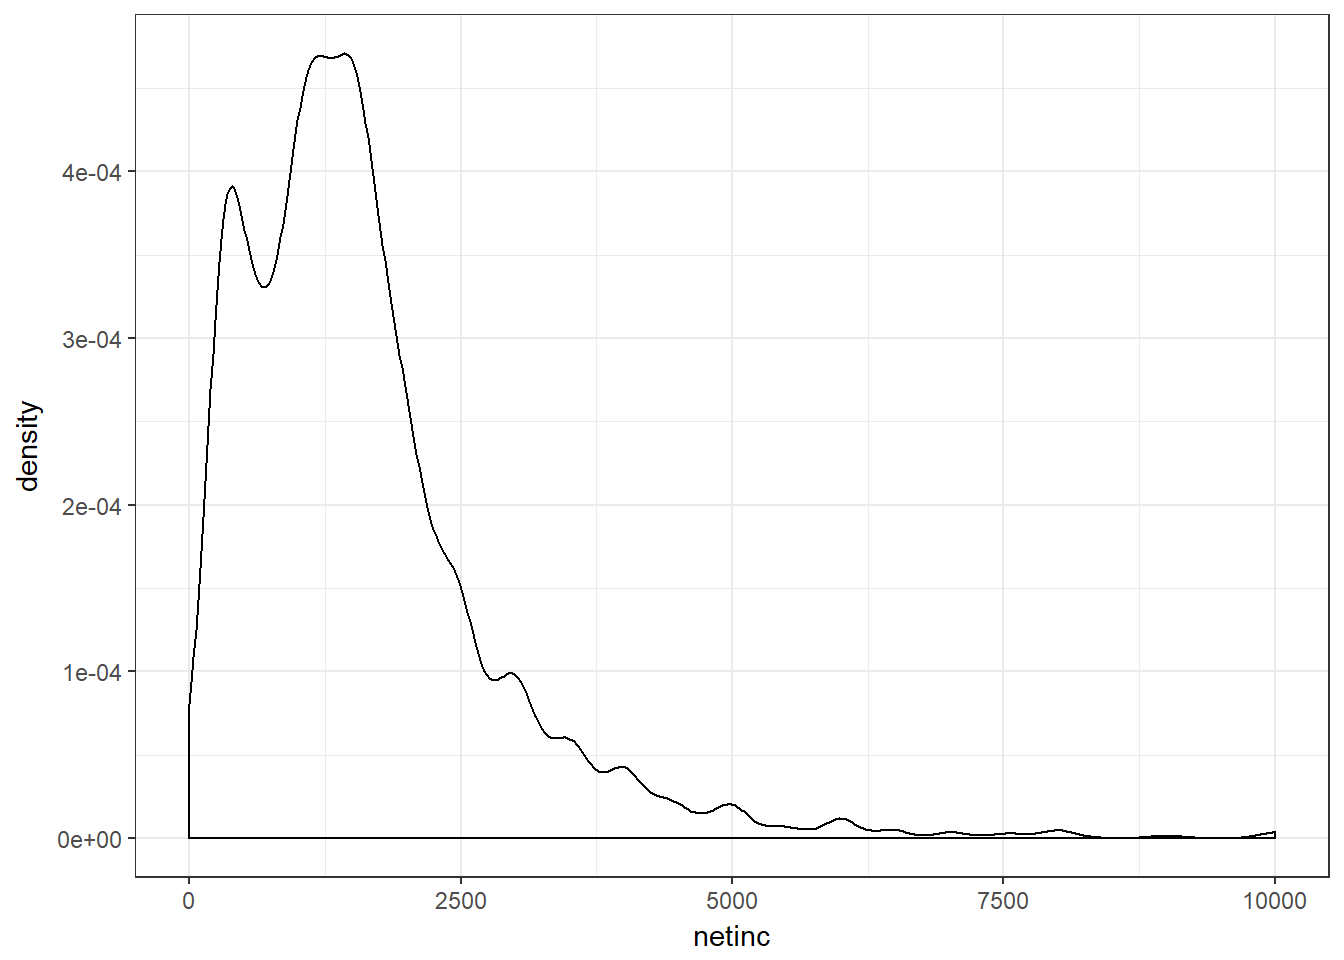
\includegraphics{hypothesis_tests_files/figure-latex/unnamed-chunk-1-1.pdf}

\subsection{Sample}\label{sample}

We draw a random sample with size \texttt{50} from our population:

\begin{Shaded}
\begin{Highlighting}[]
\KeywordTok{set.seed}\NormalTok{(}\DecValTok{24}\NormalTok{)}
\NormalTok{sample_n <-}\StringTok{ }\DecValTok{50}
\NormalTok{sample <-}\StringTok{ }\KeywordTok{sample}\NormalTok{(}\DataTypeTok{x =}\NormalTok{ inc, }\DataTypeTok{size =}\NormalTok{ sample_n, }\DataTypeTok{replace =}\NormalTok{ F)}
\end{Highlighting}
\end{Shaded}

\begin{Shaded}
\begin{Highlighting}[]
\KeywordTok{ggplot}\NormalTok{() }\OperatorTok{+}
\KeywordTok{geom_histogram}\NormalTok{(}\KeywordTok{aes}\NormalTok{(}\DataTypeTok{x =}\NormalTok{ sample,}
\DataTypeTok{y =}\NormalTok{ ..density..),}\DataTypeTok{binwidth =} \DecValTok{50}\NormalTok{,}\DataTypeTok{alpha =} \FloatTok{0.8}\NormalTok{) }\OperatorTok{+}
\KeywordTok{labs}\NormalTok{(}\DataTypeTok{title =} \StringTok{"SAMPLE Histogram Income ZU Students"}\NormalTok{) }\OperatorTok{+}
\KeywordTok{theme_minimal}\NormalTok{()}
\end{Highlighting}
\end{Shaded}

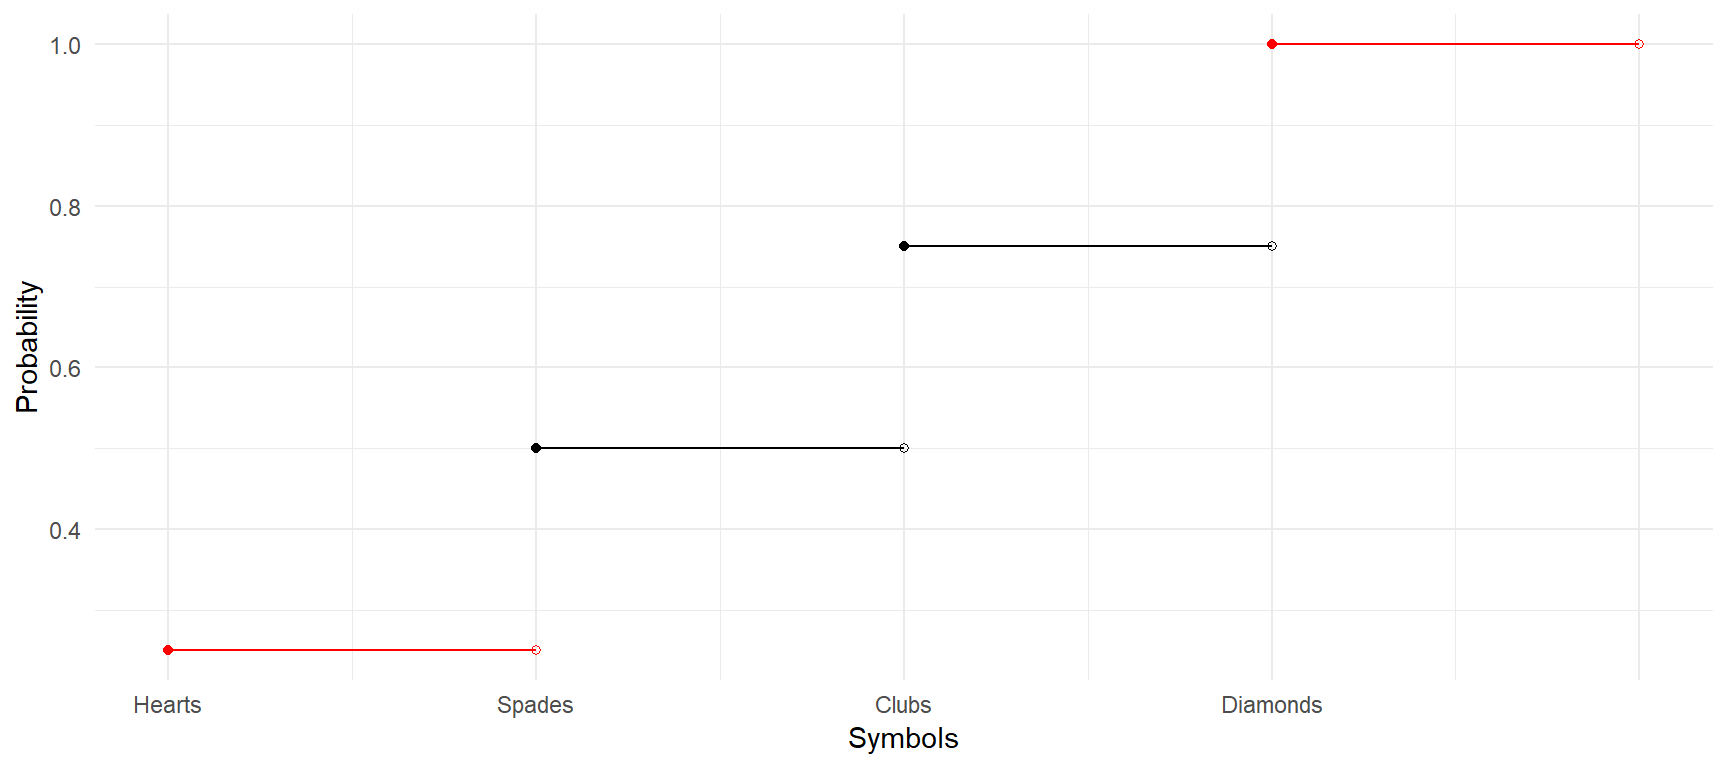
\includegraphics{hypothesis_tests_files/figure-latex/unnamed-chunk-3-1.pdf}

\section{Hypothesis Testing
Procedure}\label{hypothesis-testing-procedure}

Given the assumption that our population is distributed normally we:

\subsection{\texorpdfstring{Formulate the Null-Hypothesis that mean
student income is less then
\(940 €\)}{Formulate the Null-Hypothesis that mean student income is less then 940 \euro{}}}\label{formulate-the-null-hypothesis-that-mean-student-income-is-less-then-940}

\[ H_0 : \mu_{inc} < 940  \] Which leaves us with the alternative
Hypothesis that the mean income is more or equal to \(940€\):
\[ H_1: \mu_{inc} \geq 940 \]

\begin{Shaded}
\begin{Highlighting}[]
\NormalTok{mu_inc =}\StringTok{ }\DecValTok{940}
\NormalTok{mu_inc}
\end{Highlighting}
\end{Shaded}

\begin{verbatim}
## [1] 940
\end{verbatim}

\subsection{\texorpdfstring{Estimate the mean with the sample mean
\(\bar{X}\)}{Estimate the mean with the sample mean \textbackslash{}bar\{X\}}}\label{estimate-the-mean-with-the-sample-mean-barx}

\begin{Shaded}
\begin{Highlighting}[]
\NormalTok{inc_bar <-}\StringTok{ }\KeywordTok{mean}\NormalTok{(sample)}
\NormalTok{inc_bar}
\end{Highlighting}
\end{Shaded}

\begin{verbatim}
## [1] 998.3979
\end{verbatim}

\subsection{\texorpdfstring{Estimate the sampling standard deviation
\(S / \sqrt{n}\)}{Estimate the sampling standard deviation S / \textbackslash{}sqrt\{n\}}}\label{estimate-the-sampling-standard-deviation-s-sqrtn}

\begin{Shaded}
\begin{Highlighting}[]
\NormalTok{S_inc_bar <-}\StringTok{ }\KeywordTok{sqrt}\NormalTok{(}\KeywordTok{var}\NormalTok{(sample)}\OperatorTok{/}\NormalTok{(sample_n))}
\NormalTok{S_inc_bar}
\end{Highlighting}
\end{Shaded}

\begin{verbatim}
## [1] 27.27298
\end{verbatim}

At this state we would expect our sample mean to be distributed like
this:

\begin{Shaded}
\begin{Highlighting}[]
\KeywordTok{ggplot}\NormalTok{(}\DataTypeTok{data =}  \KeywordTok{data.frame}\NormalTok{(}\DataTypeTok{X_bar =} \DecValTok{850}\OperatorTok{:}\DecValTok{1030}\NormalTok{), }\KeywordTok{aes}\NormalTok{(}\DataTypeTok{x=}\NormalTok{X_bar)) }\OperatorTok{+}
\StringTok{  }\KeywordTok{stat_function}\NormalTok{(}\DataTypeTok{fun =}\NormalTok{ dnorm, }\DataTypeTok{args =} \KeywordTok{list}\NormalTok{(}\DataTypeTok{mean =}\NormalTok{ mu_inc, }\DataTypeTok{sd =}\NormalTok{ S_inc_bar), }\DataTypeTok{size =} \DecValTok{2}\NormalTok{) }\OperatorTok{+}
\StringTok{  }\KeywordTok{geom_vline}\NormalTok{(}\DataTypeTok{xintercept =}\NormalTok{ inc_bar, }\DataTypeTok{color =} \StringTok{"red"}\NormalTok{, }\DataTypeTok{size =} \FloatTok{1.5}\NormalTok{) }\OperatorTok{+}
\StringTok{  }\KeywordTok{geom_vline}\NormalTok{(}\DataTypeTok{xintercept =}\NormalTok{ mu_inc, }\DataTypeTok{color =} \StringTok{"green"}\NormalTok{, }\DataTypeTok{size =} \FloatTok{1.5}\NormalTok{) }\OperatorTok{+}
\StringTok{  }\KeywordTok{labs}\NormalTok{(}\DataTypeTok{title =} \StringTok{"Assumed PDF of our sample mean under H0"}\NormalTok{) }\OperatorTok{+}
\StringTok{  }\KeywordTok{theme_minimal}\NormalTok{()}
\end{Highlighting}
\end{Shaded}

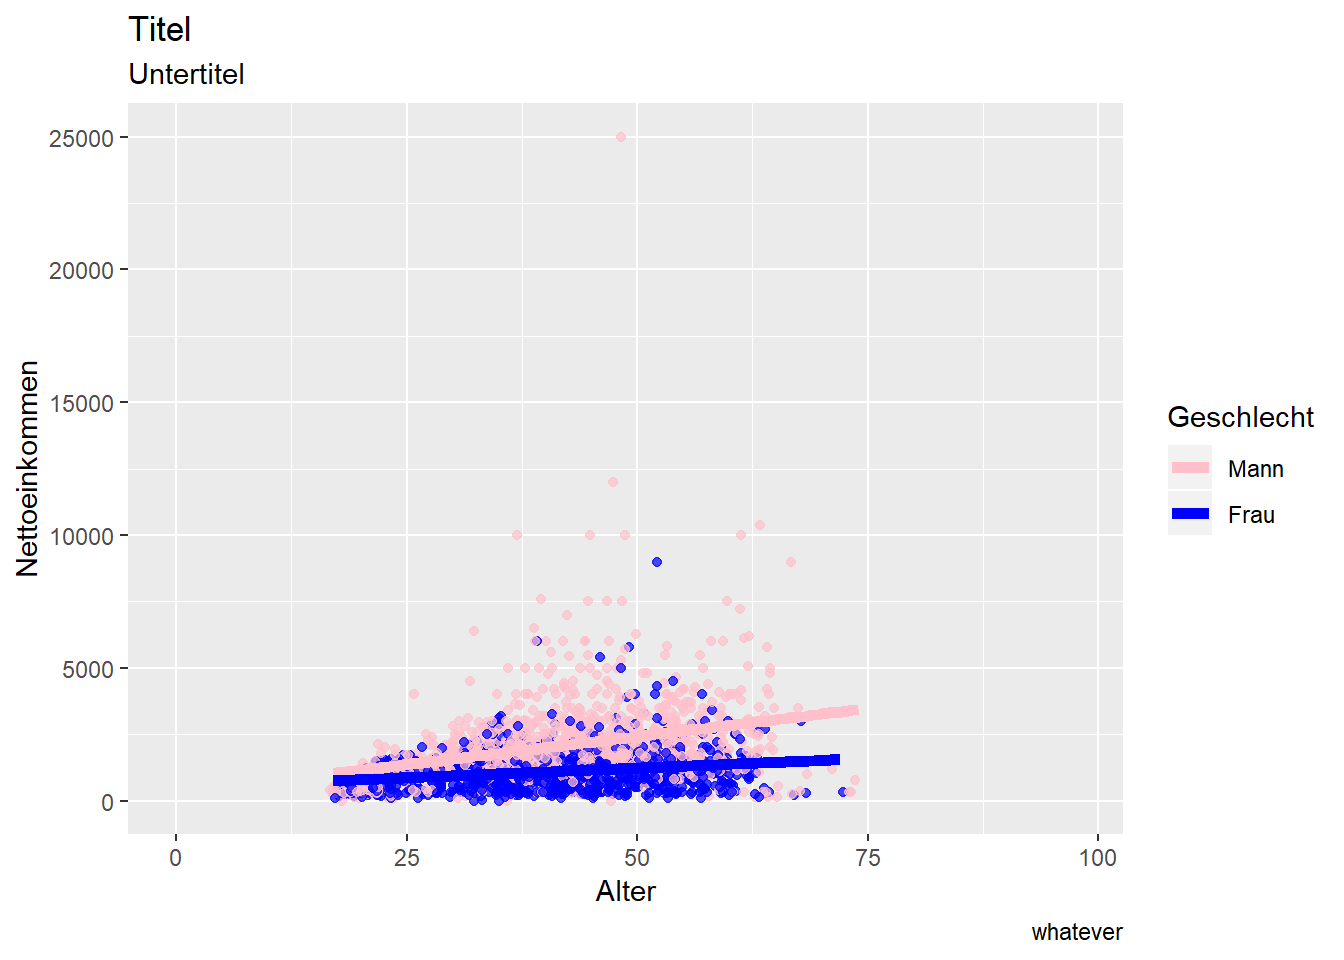
\includegraphics{hypothesis_tests_files/figure-latex/unnamed-chunk-7-1.pdf}

\subsection{\texorpdfstring{Standardise \(\bar{X}\) so we can easily
calculate
probabilities}{Standardise \textbackslash{}bar\{X\} so we can easily calculate probabilities}}\label{standardise-barx-so-we-can-easily-calculate-probabilities}

\begin{Shaded}
\begin{Highlighting}[]
\NormalTok{Z_inc_bar <-}\StringTok{ }\NormalTok{(inc_bar }\OperatorTok{-}\StringTok{ }\DecValTok{940}\NormalTok{) }\OperatorTok{/}\StringTok{ }\NormalTok{(S_inc_bar)}
\NormalTok{Z_inc_bar}
\end{Highlighting}
\end{Shaded}

\begin{verbatim}
## [1] 2.141236
\end{verbatim}

Our standardised income is also called the \emph{test statistic}.

\begin{Shaded}
\begin{Highlighting}[]
\KeywordTok{ggplot}\NormalTok{(}\DataTypeTok{data =}  \KeywordTok{data.frame}\NormalTok{(}\DataTypeTok{Z_inc_bar =} \OperatorTok{-}\DecValTok{4}\OperatorTok{:}\DecValTok{4}\NormalTok{), }\KeywordTok{aes}\NormalTok{(}\DataTypeTok{x=}\NormalTok{Z_inc_bar)) }\OperatorTok{+}
\StringTok{  }\KeywordTok{stat_function}\NormalTok{(}\DataTypeTok{fun =}\NormalTok{ dnorm, }\DataTypeTok{args =} \KeywordTok{list}\NormalTok{(}\DataTypeTok{mean =} \DecValTok{0}\NormalTok{, }\DataTypeTok{sd =} \DecValTok{1}\NormalTok{), }\DataTypeTok{size =} \DecValTok{2}\NormalTok{) }\OperatorTok{+}
\StringTok{  }\KeywordTok{geom_vline}\NormalTok{(}\DataTypeTok{xintercept =}\NormalTok{ Z_inc_bar, }\DataTypeTok{color =} \StringTok{"red"}\NormalTok{, }\DataTypeTok{size =} \FloatTok{1.5}\NormalTok{) }\OperatorTok{+}
\StringTok{  }\KeywordTok{geom_vline}\NormalTok{(}\DataTypeTok{xintercept =} \DecValTok{0}\NormalTok{, }\DataTypeTok{color =} \StringTok{"green"}\NormalTok{, }\DataTypeTok{size =} \FloatTok{1.5}\NormalTok{) }\OperatorTok{+}
\StringTok{  }\KeywordTok{labs}\NormalTok{(}\DataTypeTok{title =} \StringTok{"Assumed PDF of our standardised sample mean under H0"}\NormalTok{) }\OperatorTok{+}
\StringTok{  }\KeywordTok{theme_minimal}\NormalTok{()}
\end{Highlighting}
\end{Shaded}

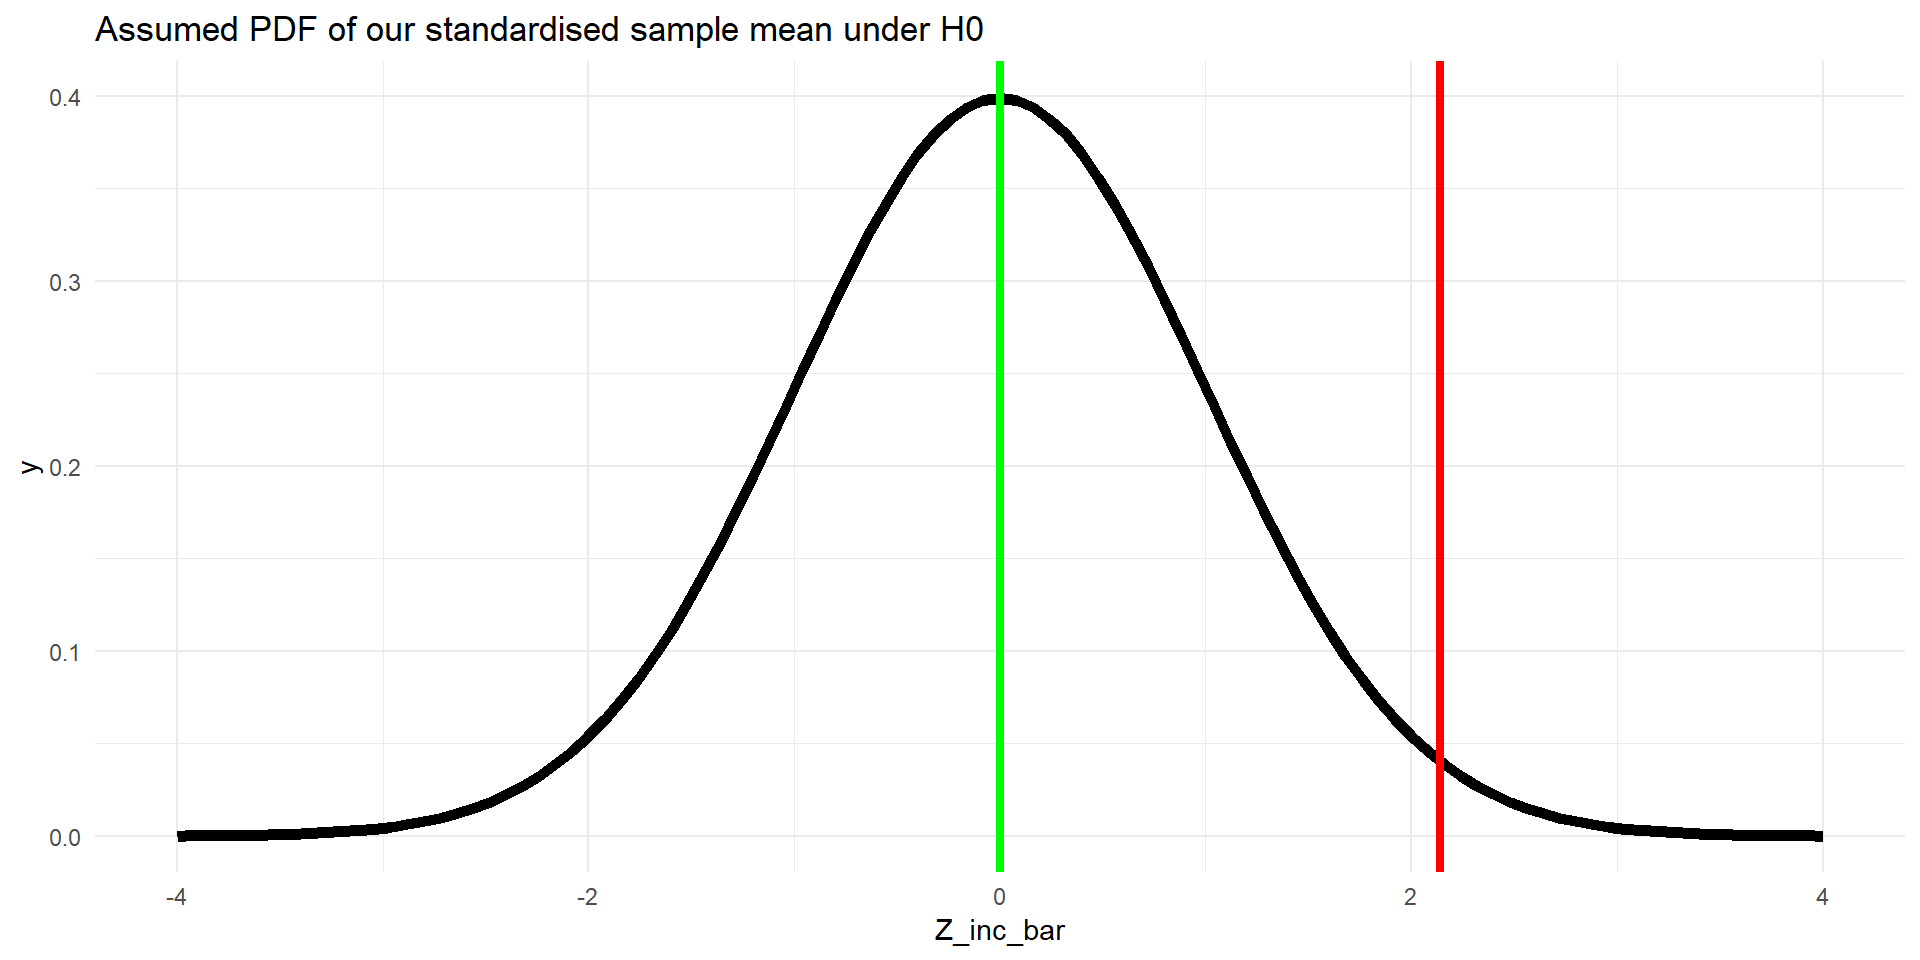
\includegraphics{hypothesis_tests_files/figure-latex/unnamed-chunk-9-1.pdf}

\subsection{\texorpdfstring{Calculate probability of \(\bar{X}\)
occuring at 5\% significance
level}{Calculate probability of \textbackslash{}bar\{X\} occuring at 5\% significance level}}\label{calculate-probability-of-barx-occuring-at-5-significance-level}

Look up the critical \(z-value\) for \(1-5\% = 95\%\), e.g.~in this
\href{http://www.z-table.com/}{table}.

\[ c = z_{95 \%} \approx 1.65 \]

Or in R:

\begin{Shaded}
\begin{Highlighting}[]
\KeywordTok{qnorm}\NormalTok{(}\FloatTok{0.95}\NormalTok{)}
\end{Highlighting}
\end{Shaded}

\begin{verbatim}
## [1] 1.644854
\end{verbatim}

Lets visualise this:

\begin{Shaded}
\begin{Highlighting}[]
\KeywordTok{ggplot}\NormalTok{(}\DataTypeTok{data =}  \KeywordTok{data.frame}\NormalTok{(}\DataTypeTok{Z_inc_bar =} \OperatorTok{-}\DecValTok{4}\OperatorTok{:}\DecValTok{4}\NormalTok{), }\KeywordTok{aes}\NormalTok{(}\DataTypeTok{x=}\NormalTok{Z_inc_bar)) }\OperatorTok{+}
\StringTok{  }\KeywordTok{stat_function}\NormalTok{(}\DataTypeTok{fun =}\NormalTok{ dnorm, }\DataTypeTok{args =} \KeywordTok{list}\NormalTok{(}\DataTypeTok{mean =} \DecValTok{0}\NormalTok{, }\DataTypeTok{sd =} \DecValTok{1}\NormalTok{), }\DataTypeTok{size =} \DecValTok{2}\NormalTok{) }\OperatorTok{+}
\StringTok{    }\KeywordTok{stat_function}\NormalTok{(}\DataTypeTok{fun =}\NormalTok{ dnorm, }\DataTypeTok{xlim =} \KeywordTok{c}\NormalTok{(}\OperatorTok{-}\DecValTok{4}\NormalTok{,}\FloatTok{1.65}\NormalTok{), }\DataTypeTok{geom =} \StringTok{"area"}\NormalTok{, }\DataTypeTok{fill =} \StringTok{"grey"}\NormalTok{, }\DataTypeTok{alpha=}\FloatTok{0.5}\NormalTok{) }\OperatorTok{+}
\StringTok{  }\KeywordTok{stat_function}\NormalTok{(}\DataTypeTok{fun =}\NormalTok{ dnorm, }\DataTypeTok{xlim =} \KeywordTok{c}\NormalTok{(}\FloatTok{1.65}\NormalTok{,}\DecValTok{4}\NormalTok{), }\DataTypeTok{geom =} \StringTok{"area"}\NormalTok{, }\DataTypeTok{fill =} \StringTok{"black"}\NormalTok{, }\DataTypeTok{alpha=}\FloatTok{0.5}\NormalTok{) }\OperatorTok{+}
\StringTok{  }\KeywordTok{geom_vline}\NormalTok{(}\DataTypeTok{xintercept =}\NormalTok{ Z_inc_bar, }\DataTypeTok{color =} \StringTok{"red"}\NormalTok{, }\DataTypeTok{size =} \FloatTok{1.5}\NormalTok{) }\OperatorTok{+}
\StringTok{  }\KeywordTok{geom_vline}\NormalTok{(}\DataTypeTok{xintercept =} \DecValTok{0}\NormalTok{, }\DataTypeTok{color =} \StringTok{"green"}\NormalTok{, }\DataTypeTok{size =} \FloatTok{1.5}\NormalTok{) }\OperatorTok{+}
\StringTok{  }\KeywordTok{labs}\NormalTok{(}\DataTypeTok{title =} \StringTok{"Assumed PDF of our standardised sample mean under H0"}\NormalTok{) }\OperatorTok{+}
\StringTok{  }\KeywordTok{theme_minimal}\NormalTok{()}
\end{Highlighting}
\end{Shaded}

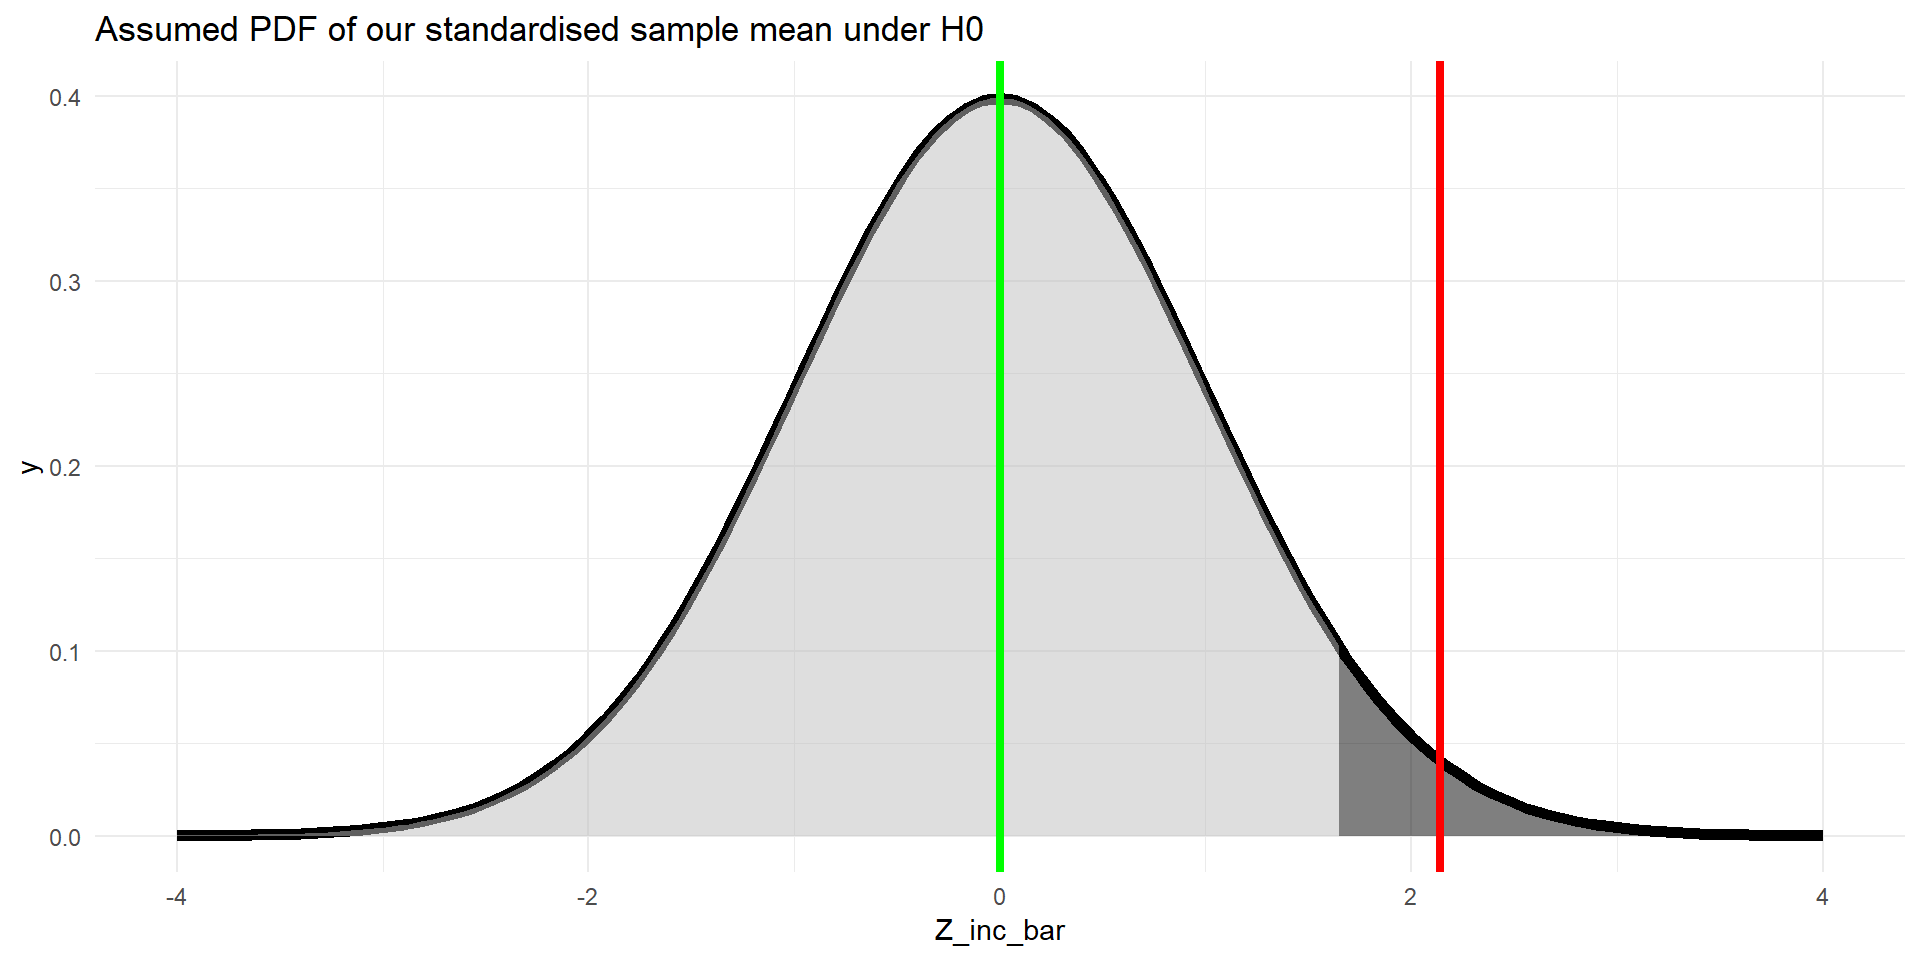
\includegraphics{hypothesis_tests_files/figure-latex/unnamed-chunk-11-1.pdf}

\subsubsection{Hypothesis Test:}\label{hypothesis-test}

Check whether our standardised estimator \(Z_{\bar{inc}}\) is larger
than our critical value \(c\).

\begin{itemize}
\tightlist
\item
  Critical value \(c\): quantile of the standard normal cdf with
  \(P(z > c) = 95 \%\)
\item
  Test statistic: our standardised estimator \(Z_{\bar{inc}}\)
\end{itemize}

Remember our \(H_0: \mu_{inc} < 940€\) and \(H_1: \mu_{inc} \geq 940€\).
Lets test that in R:

\begin{Shaded}
\begin{Highlighting}[]
\NormalTok{Z_inc_bar }\OperatorTok{>=}\StringTok{ }\KeywordTok{qnorm}\NormalTok{(}\FloatTok{0.95}\NormalTok{)}
\end{Highlighting}
\end{Shaded}

\begin{verbatim}
## [1] TRUE
\end{verbatim}

We now can make the following statements:

\begin{itemize}
\tightlist
\item
  If the \(H_0\) is true, samples with a \(Z_\bar{inc}\) in the dark
  grey area only occur \(5\%\) of the time

  \begin{itemize}
  \tightlist
  \item
    We call that area the rejection region
  \end{itemize}
\item
  We showed that our observed sample mean (in standardised form) falls
  into the rejection region
\item
  In conclusion, we have some evidence against our initial assumption
  that mean student income is at most \(940 €\)
\item
  This means that we can be optimistic that our sample is not one of the
  \(5 \%\) of outliers in the world of \(H_0\), but that the \(H_0\) is
  wrong
\end{itemize}

Generally we can make the statement: ``we can reject the null hypothesis
that mean ZU student income is less than \(940€\) at a significance
level of \(5\%\)''

\subsubsection{Hypothesis Test - Other Possible
Variants}\label{hypothesis-test---other-possible-variants}

What we did was only the \emph{right-sided} hypothesis test.

We could also test other hypotheses:

\begin{itemize}
\tightlist
\item
  Left-sided: \(H_0: \mu_{inc} > 940€\) and \(H_1: \mu_{inc} \leq 940€\)

  \begin{itemize}
  \tightlist
  \item
    Test: \(\mu_{inc} \leq c\)
  \end{itemize}
\item
  Both-sided: \(H_0: \mu_{inc} = 940€\) and \(H_1: \mu_{inc} \neq 940€\)

  \begin{itemize}
  \tightlist
  \item
    Test :\(|\mu_{inc}| > c\)
  \end{itemize}
\end{itemize}

\subsection{P-Values}\label{p-values}

So called \emph{p-values} are often used and reported in statistical
work. They indicate the highest level of significance at which we can
reject the \(H_0\).

In our example, we could not only reject the \(H_0\) at the \(5\%\)
level, but also at the \(2.5\%\) level:

\begin{Shaded}
\begin{Highlighting}[]
\KeywordTok{ggplot}\NormalTok{(}\DataTypeTok{data =}  \KeywordTok{data.frame}\NormalTok{(}\DataTypeTok{Z_inc_bar =} \OperatorTok{-}\DecValTok{4}\OperatorTok{:}\DecValTok{4}\NormalTok{), }\KeywordTok{aes}\NormalTok{(}\DataTypeTok{x=}\NormalTok{Z_inc_bar)) }\OperatorTok{+}
\StringTok{  }\KeywordTok{stat_function}\NormalTok{(}\DataTypeTok{fun =}\NormalTok{ dnorm, }\DataTypeTok{args =} \KeywordTok{list}\NormalTok{(}\DataTypeTok{mean =} \DecValTok{0}\NormalTok{, }\DataTypeTok{sd =} \DecValTok{1}\NormalTok{), }\DataTypeTok{size =} \DecValTok{2}\NormalTok{) }\OperatorTok{+}
\StringTok{    }\KeywordTok{stat_function}\NormalTok{(}\DataTypeTok{fun =}\NormalTok{ dnorm, }\DataTypeTok{xlim =} \KeywordTok{c}\NormalTok{(}\OperatorTok{-}\DecValTok{4}\NormalTok{,}\FloatTok{1.65}\NormalTok{), }\DataTypeTok{geom =} \StringTok{"area"}\NormalTok{, }\DataTypeTok{fill =} \StringTok{"grey"}\NormalTok{, }\DataTypeTok{alpha=}\FloatTok{0.5}\NormalTok{) }\OperatorTok{+}
\StringTok{  }\KeywordTok{stat_function}\NormalTok{(}\DataTypeTok{fun =}\NormalTok{ dnorm, }\DataTypeTok{xlim =} \KeywordTok{c}\NormalTok{(}\FloatTok{1.65}\NormalTok{,}\FloatTok{1.96}\NormalTok{), }\DataTypeTok{geom =} \StringTok{"area"}\NormalTok{, }\DataTypeTok{fill =} \StringTok{"darkgrey"}\NormalTok{, }\DataTypeTok{alpha=}\FloatTok{0.5}\NormalTok{) }\OperatorTok{+}
\StringTok{  }\KeywordTok{stat_function}\NormalTok{(}\DataTypeTok{fun =}\NormalTok{ dnorm, }\DataTypeTok{xlim =} \KeywordTok{c}\NormalTok{(}\FloatTok{1.96}\NormalTok{,}\DecValTok{4}\NormalTok{), }\DataTypeTok{geom =} \StringTok{"area"}\NormalTok{, }\DataTypeTok{fill =} \StringTok{"black"}\NormalTok{, }\DataTypeTok{alpha=}\FloatTok{0.5}\NormalTok{) }\OperatorTok{+}
\StringTok{  }\KeywordTok{geom_vline}\NormalTok{(}\DataTypeTok{xintercept =}\NormalTok{ Z_inc_bar, }\DataTypeTok{color =} \StringTok{"red"}\NormalTok{, }\DataTypeTok{size =} \FloatTok{1.5}\NormalTok{) }\OperatorTok{+}
\StringTok{  }\KeywordTok{geom_vline}\NormalTok{(}\DataTypeTok{xintercept =} \DecValTok{0}\NormalTok{, }\DataTypeTok{color =} \StringTok{"green"}\NormalTok{, }\DataTypeTok{size =} \FloatTok{1.5}\NormalTok{) }\OperatorTok{+}
\StringTok{  }\KeywordTok{labs}\NormalTok{(}\DataTypeTok{title =} \StringTok{"Assumed PDF of our standardised sample mean under H0"}\NormalTok{) }\OperatorTok{+}
\StringTok{  }\KeywordTok{theme_minimal}\NormalTok{()}
\end{Highlighting}
\end{Shaded}

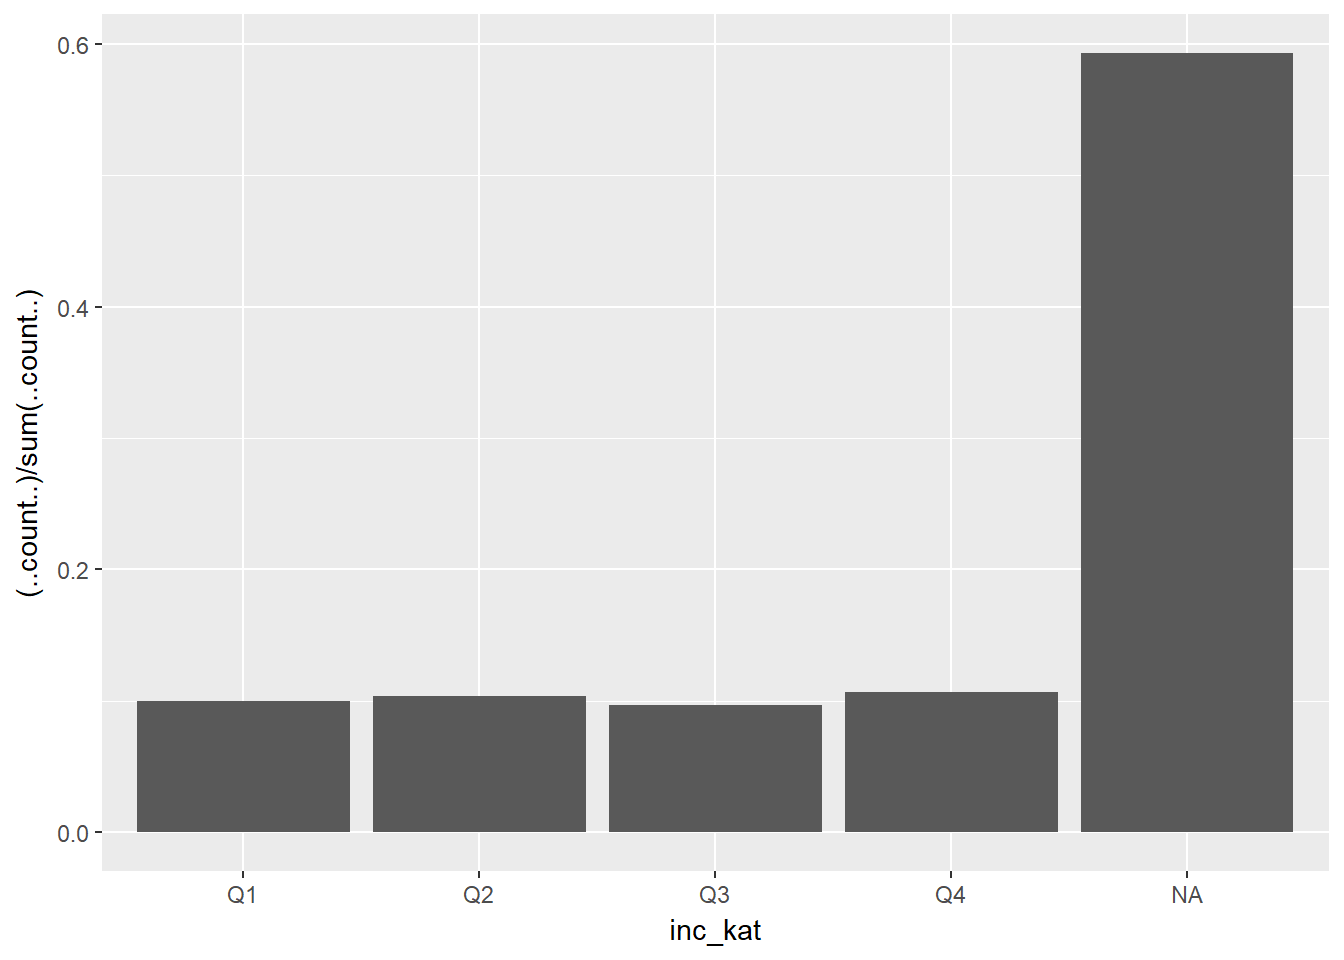
\includegraphics{hypothesis_tests_files/figure-latex/unnamed-chunk-13-1.pdf}

But at most, we could reject it at the level of our test-statistic. So
we just need to look up the corresponding value for \(Z_\bar{inc}\) in
the \href{http://www.z-table.com/}{z- table} or with r:

\begin{Shaded}
\begin{Highlighting}[]
\DecValTok{1}\OperatorTok{-}\StringTok{ }\KeywordTok{pnorm}\NormalTok{(Z_inc_bar)}
\end{Highlighting}
\end{Shaded}

\begin{verbatim}
## [1] 0.01612751
\end{verbatim}

This is our p-value. It tells us that we can reject the \(H_0\) at most
at a significance level of \(\approx 1.6 \%\).

\section{T-Test Function in R}\label{t-test-function-in-r}

In R we can conduct this procedure with the \texttt{t.test} function:

\begin{Shaded}
\begin{Highlighting}[]
\KeywordTok{t.test}\NormalTok{(sample, }\DataTypeTok{mu =} \DecValTok{940}\NormalTok{, }\DataTypeTok{alternative =} \StringTok{"greater"}\NormalTok{)}
\end{Highlighting}
\end{Shaded}

\begin{verbatim}
## 
##  One Sample t-test
## 
## data:  sample
## t = 2.1412, df = 49, p-value = 0.01863
## alternative hypothesis: true mean is greater than 940
## 95 percent confidence interval:
##  952.6733      Inf
## sample estimates:
## mean of x 
##  998.3979
\end{verbatim}

The different p-value is due to the fact that \texttt{t.test} used the
\textbf{Students t-distribution} instead of the standard normal
distribution. We used the standard normal for ease of explanation, but
actually our test statistic is distributed in the Student-t way.

If we calculate our p-value for the Student-t distribution, we get the
same result:

\begin{Shaded}
\begin{Highlighting}[]
\DecValTok{1}\OperatorTok{-}\StringTok{ }\KeywordTok{pt}\NormalTok{(Z_inc_bar, }\DecValTok{49}\NormalTok{) }\CommentTok{# degrees of freedom = sample size -1 }
\end{Highlighting}
\end{Shaded}

\begin{verbatim}
## [1] 0.01862729
\end{verbatim}

For large samples (\(n > 120\)) the t-distribution and the standard
normal distribution are almost equivalent.


\end{document}
